\documentclass[a4paper, 12pt]{article}
\usepackage{titling}
\usepackage{array}
\usepackage{booktabs}
\usepackage{enumitem}
\usepackage{graphicx}
\usepackage{subfigure}
\usepackage{hyperref}
\usepackage{amssymb}
\usepackage{listings}
\setlength{\heavyrulewidth}{1.5pt}
\setlength{\abovetopsep}{4pt}
\setlength{\parindent}{0pt}
\graphicspath{{.}}
\usepackage{color}

\usepackage[margin=1in]{geometry}

% Must be after geometry
\usepackage{fancyhdr}
\pagestyle{fancy}
\fancyhf{}
\rhead{ECTA Homework 2}
\cfoot{\thepage}

\setlength{\droptitle}{-5em}

\title{Evolutionary Computation Theory and Application  \\
				- Assignment 2: Traveling Salesman Problem -}
\author{\color{blue}Erick Kramer, Mihir Patil\\ \texttt{\color{blue}erick.romero@smail.inf.h-brs.de , mihir.patil@smail.inf.h-brs.de}}
\date{\today}

\begin{document}

\maketitle

\section{General Remarks }

Please Follow those remarks. Deviating will lead to a reduced score

\begin{itemize}
	\item label your axis 
	\item Include a descriptive, not covering legend in your plots
	\item Caption you images with a clear description
	\item Remember to name the file correctly
	\item Make sure that both team members submit the same file, with the same name
	\item Please make sure that all figures and lines are clearly readable
\end{itemize}
\newpage
\section{Solution}


\begin{table} [h!]
	  \centering
\begin{tabular}{|l|l|}
\hline
\textbf{Parameter} & \textbf{Value}   \\
\hline
Population size & 50 \\
\hline
Crossover Rates &  1\%, 10\%, 80\%, 99\% \\
\hline
Mutation Rates &  1\%, 10\%, 80\%, 99\% \\
\hline
Repetitions & 30 \\
\hline
Generations & 1000 \\
\hline
Average best fitness		 & (Shown in plots) \\
\hline
\end{tabular}
\caption{Table describing all relevant parameters for your experiments. }
\label{table:defparams}
\end{table}

\newpage
\section{Results}

\begin{figure}[h!]
  \centering
  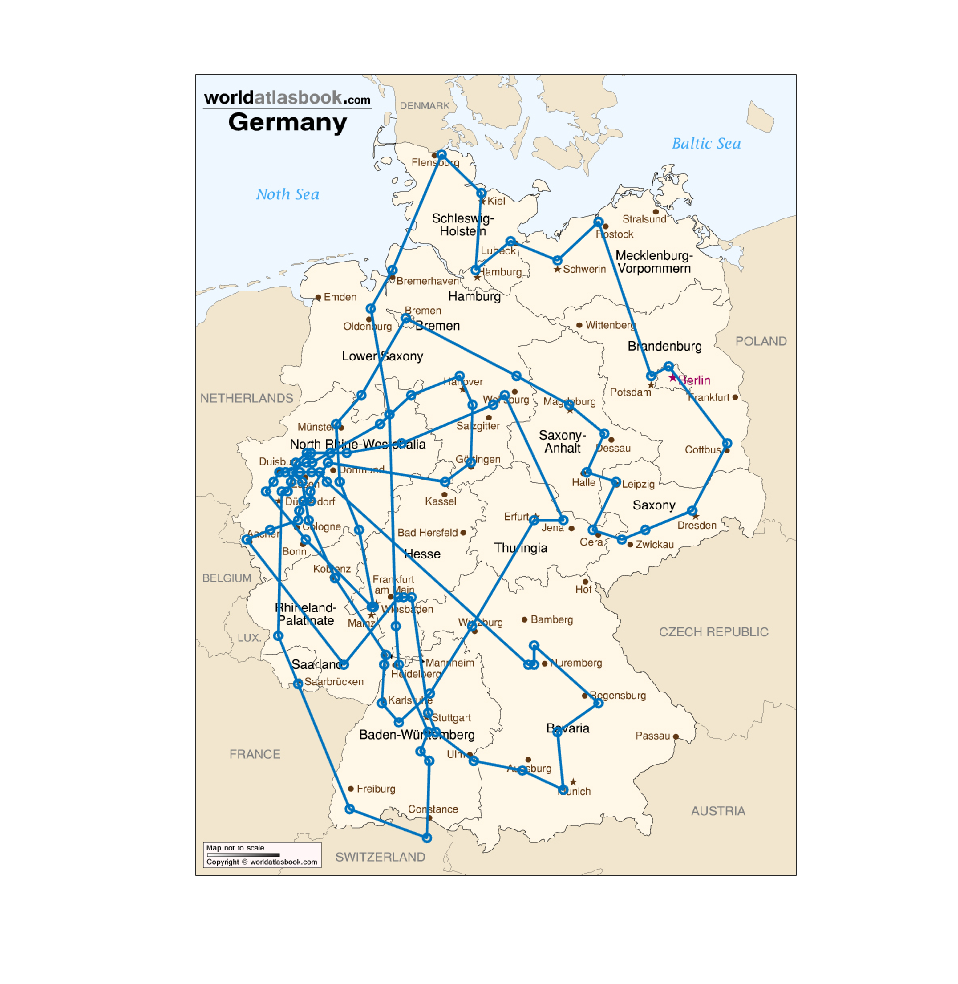
\includegraphics[width=0.4\textwidth]{images/one_run_cross_80_mut_80_50000_ind.png}
  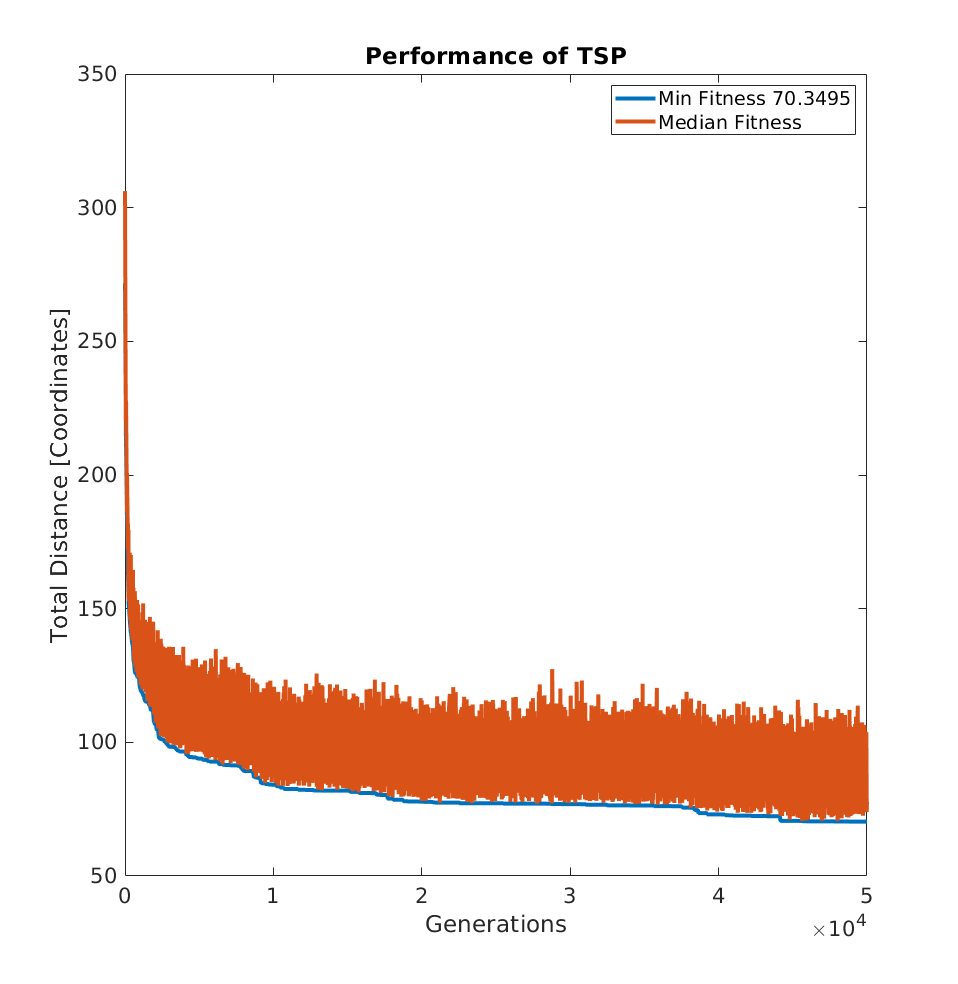
\includegraphics[width=0.4\textwidth]{images/one_run_cross_80_mut_80_50000.png}
    \caption{Best result having 50,000 generations and crossover rate of 80\% and mutation rate of 80\%. \label{fig:xxx1}}
\end{figure}

\newpage
\subsection{Different mutation rates}


\begin{figure}[h!]
	\centering
	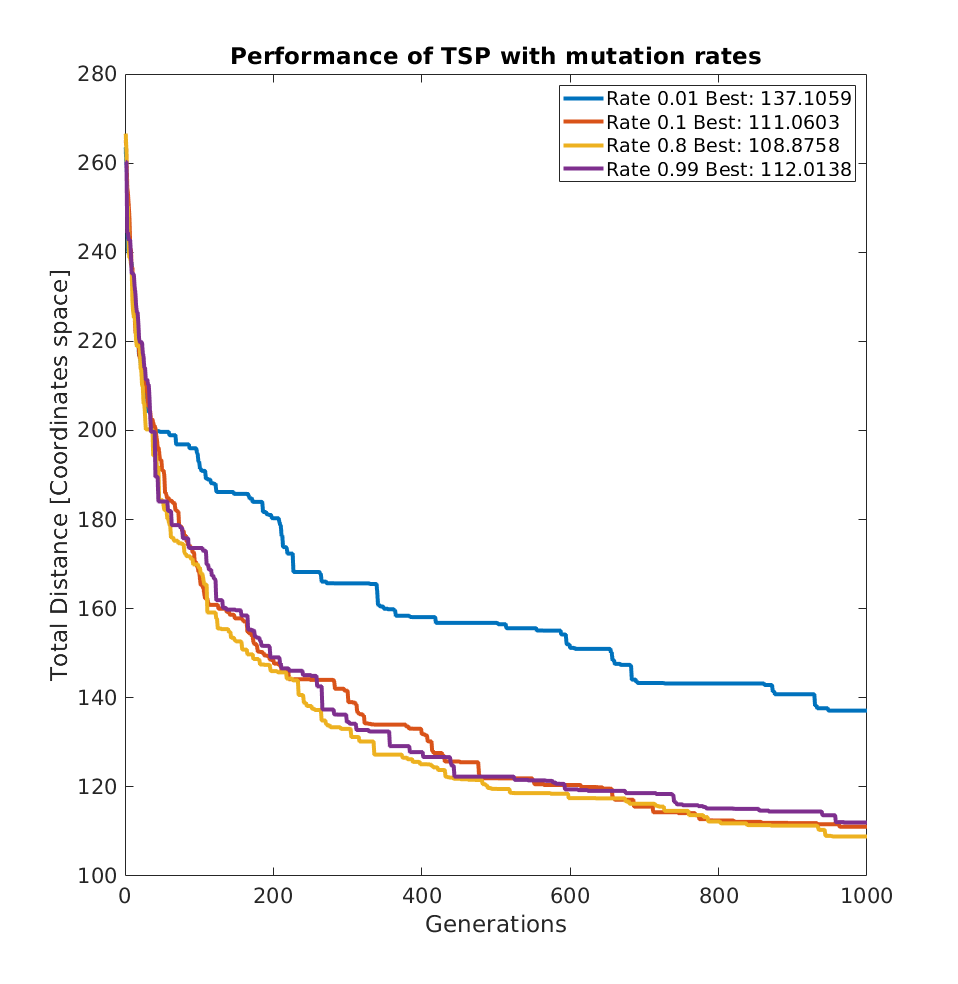
\includegraphics[width=1.0\textwidth]{images/MutationRatesVsCrossoverRate_80.png}
	\caption{Fitness plot of having different mutation rates with a fixed mutation rate of 80\%. The best fitness value for each mutation rate is shown next to the label. \label{fig:crossfig}}
\end{figure}

Describe and explain the different mutation rates and how they influence the learning behaviour. Please remember to also focus on why, not only on what.
Also elaborate on the mutation rate you have chosen as best mutation rate.

\newpage

\subsection{Different crossover rates}


\begin{figure}[h!]
	\centering
	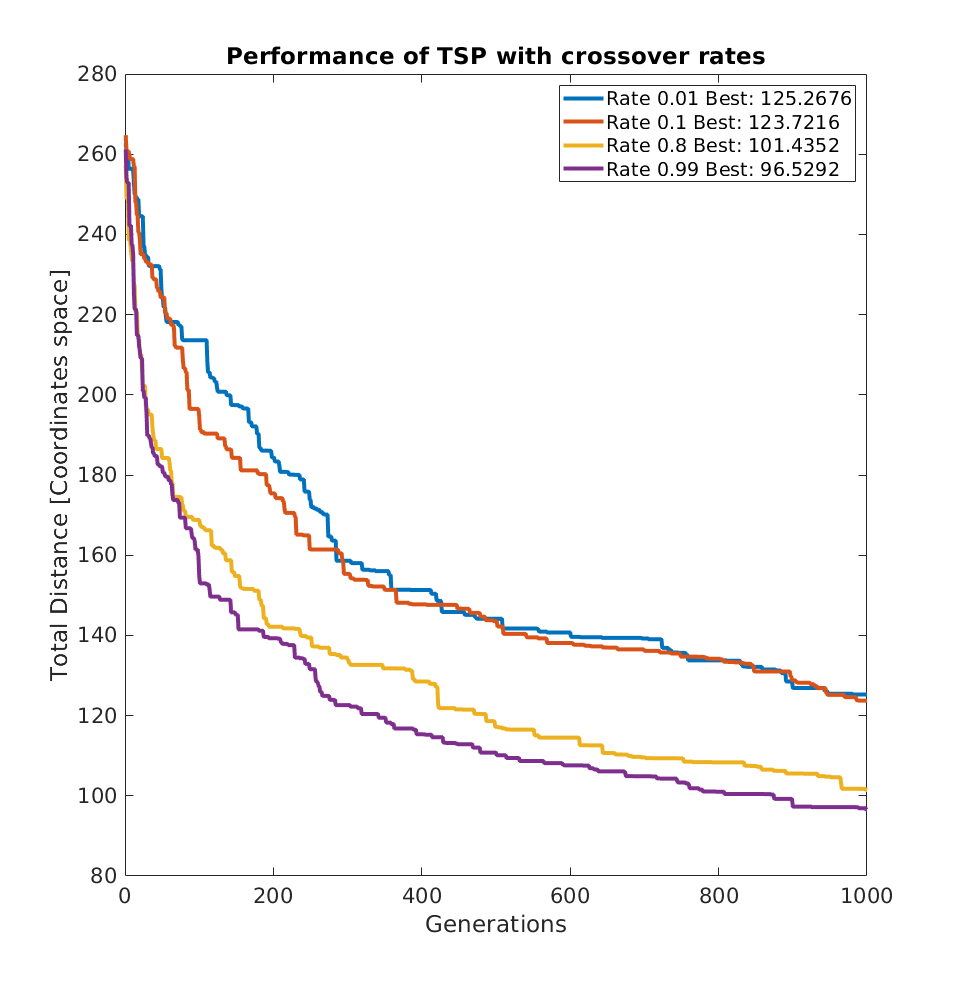
\includegraphics[width=1.0\textwidth]{images/CrossOverRatesVsMutationRate_80.png}
	\caption{Fitness plot of having different crossover rates with a fixed mutation rate of 80\%. The best fitness value for each crossover rate is shown next to the label. \label{fig:crossfig}}
\end{figure}

Describe and explain the different crossover rates and how they influence the learning behaviour. Please remember to also focus on why, not only on what.
Also elaborate on the crossover rate you have chosen as best mutation rate.
\newpage
\subsection{Comparing Algorithms}
\newpage

\begin{figure}[h!]
	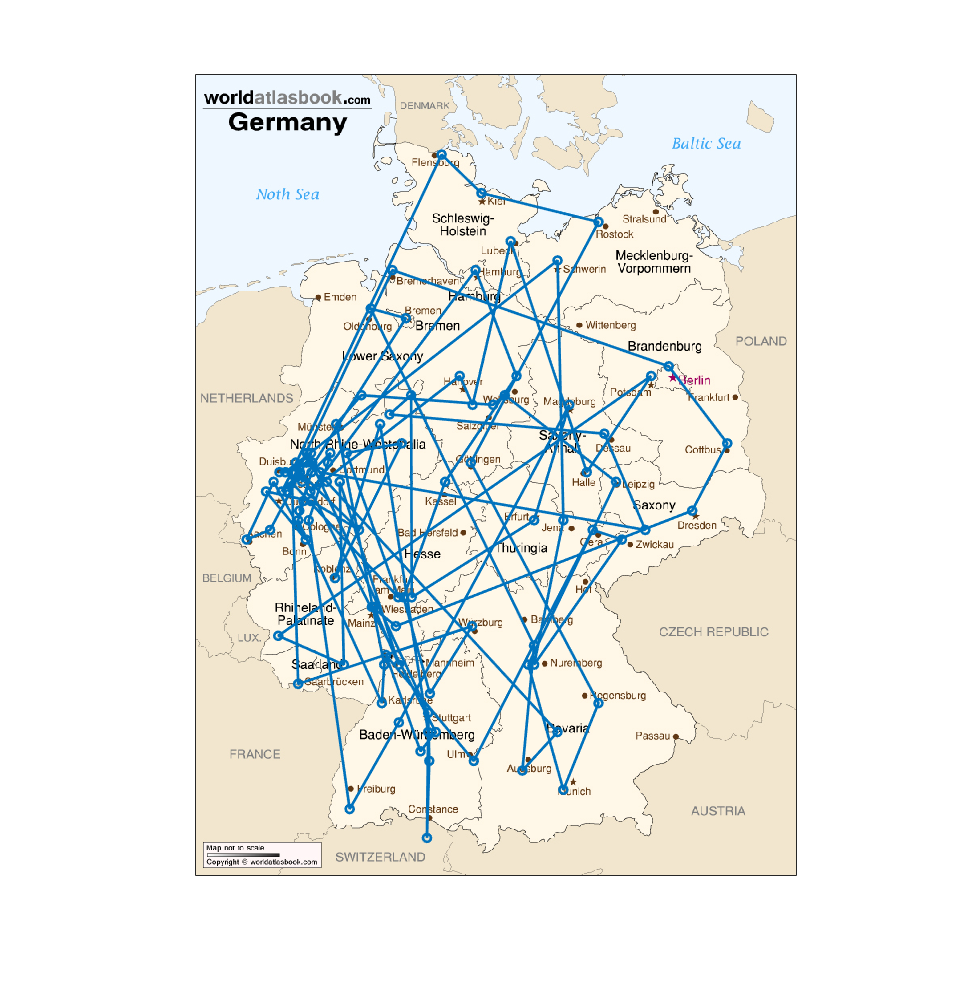
\includegraphics[width=0.5\textwidth]{images/one_point_30_runs_ind.png}
	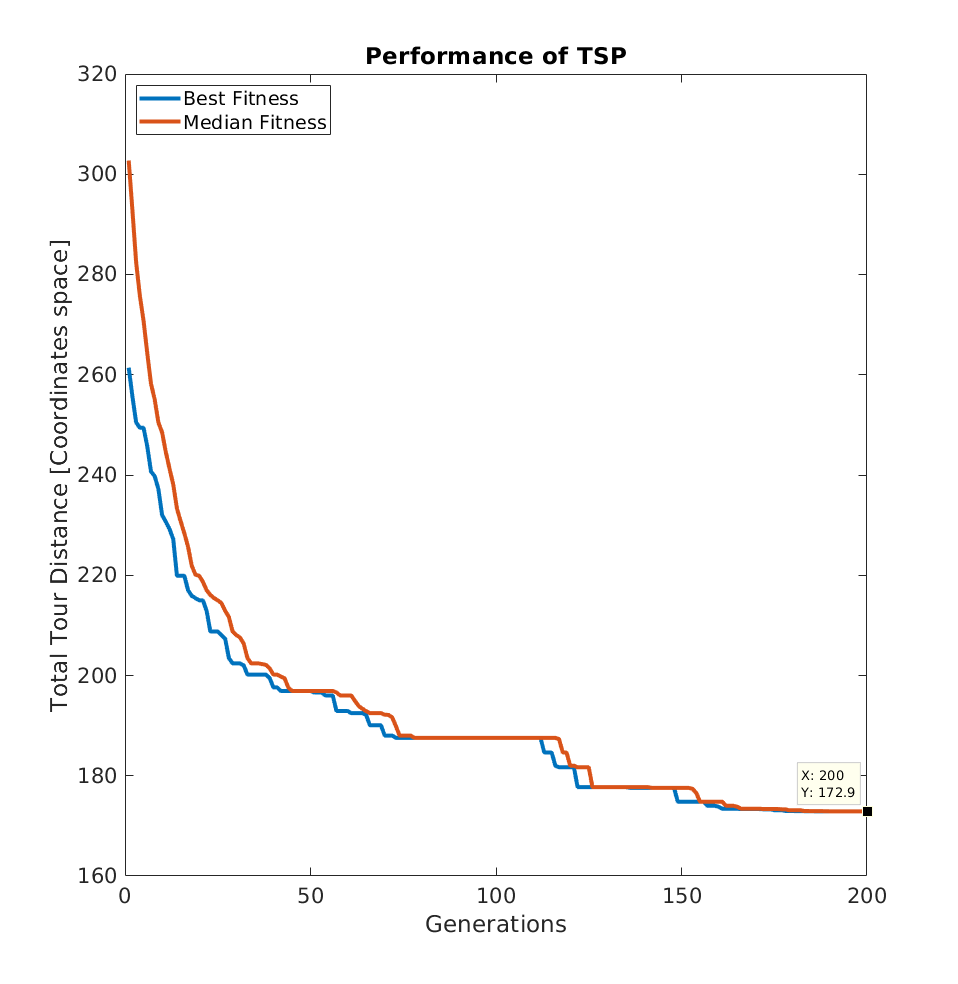
\includegraphics[width=0.5\textwidth]{images/one_point_30_runs_fit_med.png}
	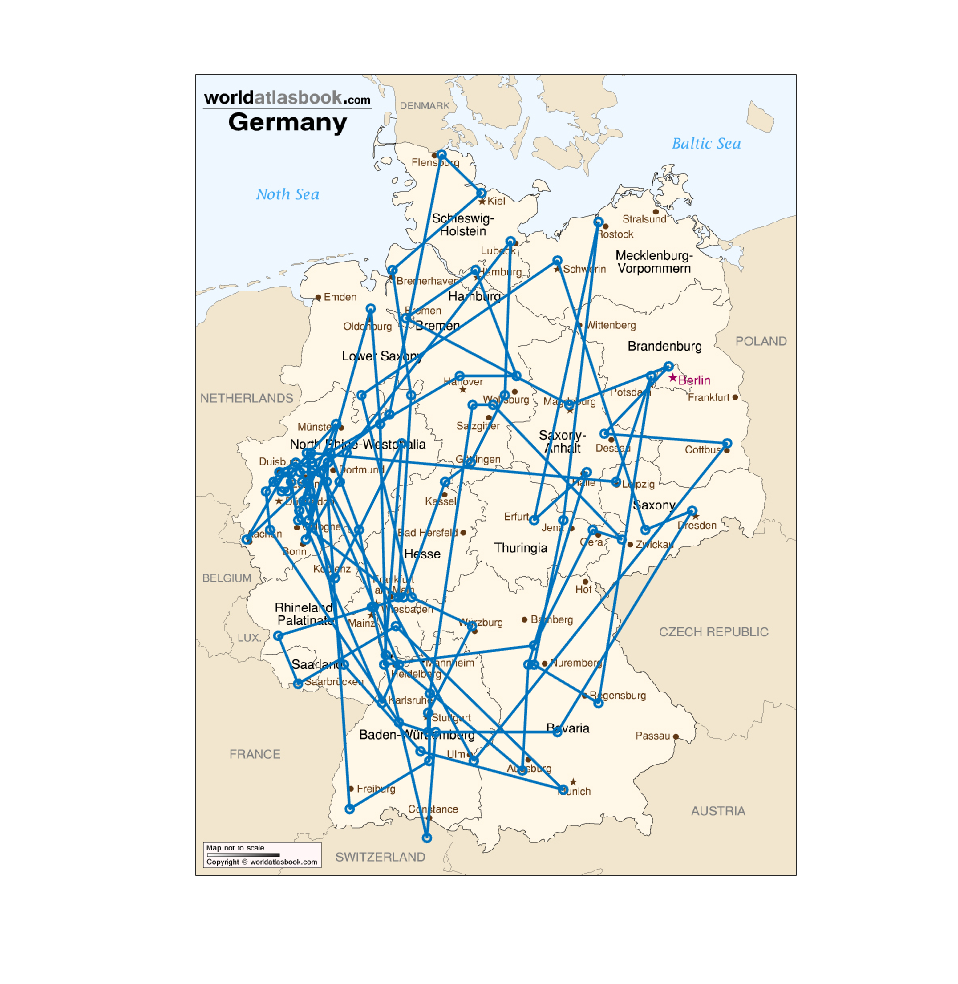
\includegraphics[width=0.5\textwidth]{images/two_points_30_runs_ind.png}
	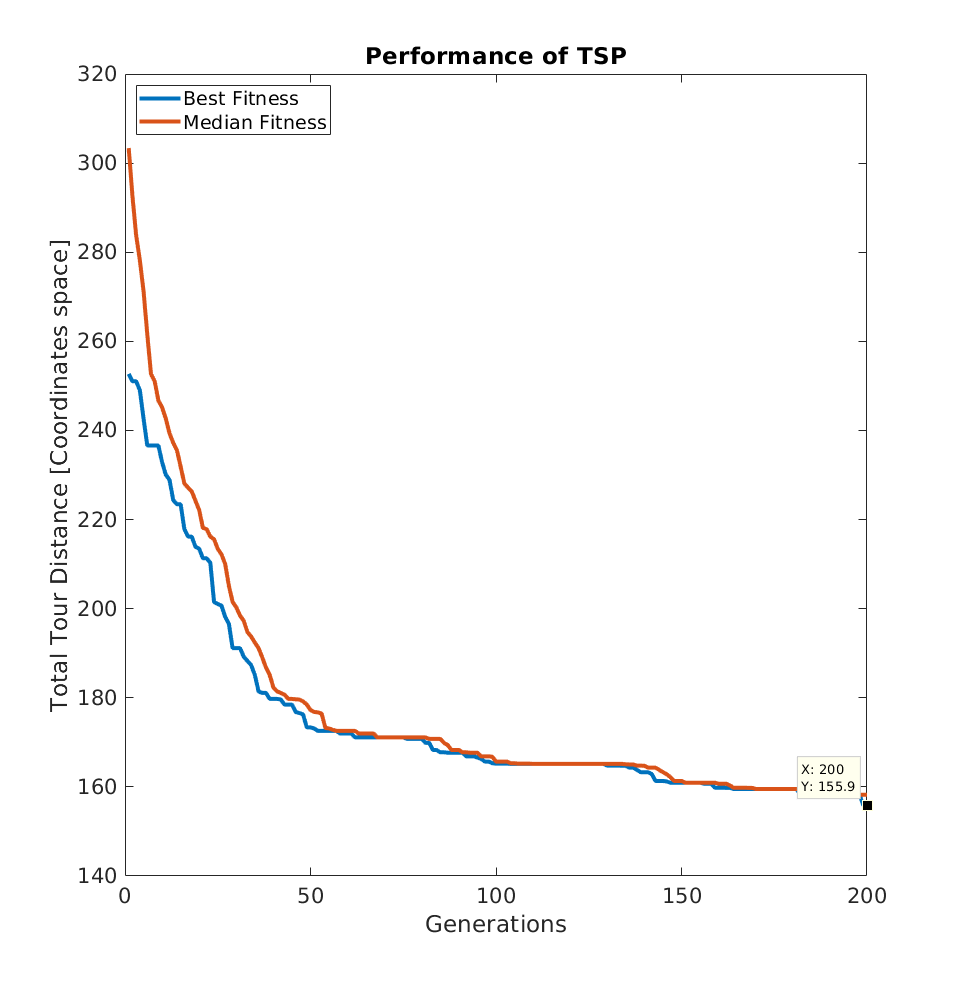
\includegraphics[width=0.5\textwidth]{images/two_points_30_runs_fit_med.png}
	\caption
	{	
		\textbf{One point vs two point crossover with 30 runs having crossover of 80\% and mutation of 30\%.}\newline
		\textit{Top Left:} One point crossover best individual,
		\textit{Top Right:} One point crossover fitness and median, 
		\textit{Bottom Left:} Two point crossover best individual, 
		\textit{Bottom Right:} Two point crossover fitness and median
	}
\end{figure}



\end{document}
